\Chapter{Tesztelés}

\Section{Reguláris kifejezések}

A reguláris kifejezések illesztését megvalósító algoritmusok gyakran eltérnek, a szerzők másként értelmeznek bizonyos eseteket, vagyis nincs egységes szabvány belőle.

Ennek ellenőrzésére érdekében konzulensemmel készítettünk egységtesztet CMocka függvénykönytvár segítségével. (Ez egy egységtesztek írásához készített függvénykönyvtár C nyelvre \cite{andreas2014cmocka}.) Amennyiben a tesztelésünk sikeres volt, és a reguláris kifejezés sablonunk megfelelően illeszkedik az adott sorra, abban az esetben teszt futtatás után a következő kimenetet kell kapjuk:
\begin{python}
[==========] Running 7 test(s).
[ RUN      ] test_vertex_line
[       OK ] test_vertex_line
[ RUN      ] test_texture_vertex_line
[       OK ] test_texture_vertex_line
[ RUN      ] test_vertex_normal_line
[       OK ] test_vertex_normal_line
[ RUN      ] test_face_line
[       OK ] test_face_line
[ RUN      ] test_triangle_line
[       OK ] test_triangle_line
[ RUN      ] test_quad_line
[       OK ] test_quad_line
[ RUN      ] test_polygon_line
[       OK ] test_polygon_line
[==========] 7 test(s) run.
[  PASSED  ] 7 test(s).
\end{python}
Abban az esetben, ha a tesztünk valamelyik fázisban elbukott, akkor a következővel tér vissza a teszt:
\begin{python}
[ RUN      ] test_quad_line
[  ERROR   ] --- result
[   LINE   ] --- tests/regex_tests.h:72: error: Failure!
[  FAILED  ] test_quad_line
[==========] 7 test(s) run.
[  PASSED  ] 6 test(s).
[  FAILED  ] 1 test(s), listed below:
[  FAILED  ] test_quad_line
\end{python}
Ennél a példánál a \texttt{QUAD\_LINE\_PATTERN} nem megfelelően illeszkedett  a tesztben megadott formátumra, ezért hibával tér vissza.

\Section{Modell betöltés sebességmérés}

\begin{figure}[h]
\centering
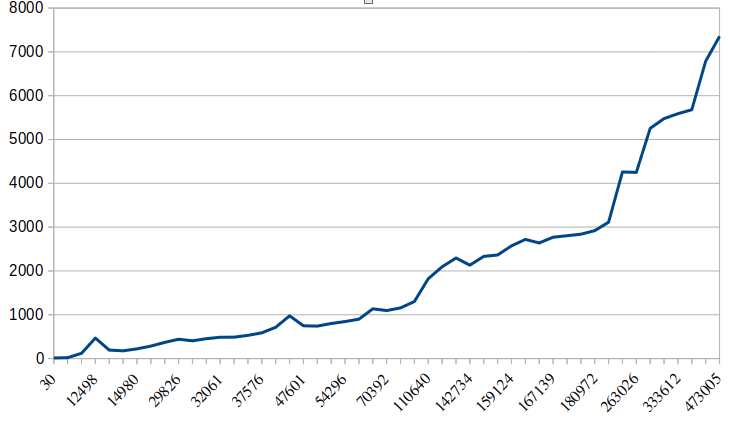
\includegraphics[width=\textwidth]{images/betoltesiido.png}
\caption{Modell betöltési idő grafikon.}
\label{fig:betolt}
\end{figure}

Modellek betöltési sebességét vizsgáltam \aref{fig:betolt}. grafikonon. A vízszintes tengelyen a modellek összes elemszáma (geometria csúcs, textúra koordináta, normál csúcs, lap elem) számok összesítése látható, a függőleges tengelyen pedig a betöltési idő milliszekundumban. Az összehasonlítás textúra, modell kirajzolás, és az OBJ fájlon történő bármilyen változtatás nélkül történt.

A grafikonon jól látható, hogy az idő növekedése közel exponenciális, tehát a modellek elemszámának növekedésének mértéke közel arányos a beolvasáshoz szükséges idő nagyságával.

\Section{Modell betöltés sebességmérés az egyes részeken}

\Aref{fig:betolt2}. diagramon látható modell betöltés a különböző részekre lebontva. Vízszintes tengelyen kapott helyet a modellek összes elemszáma. Függőleges tengelyen az idő milliszekundumban.

\begin{figure}[h]
\centering
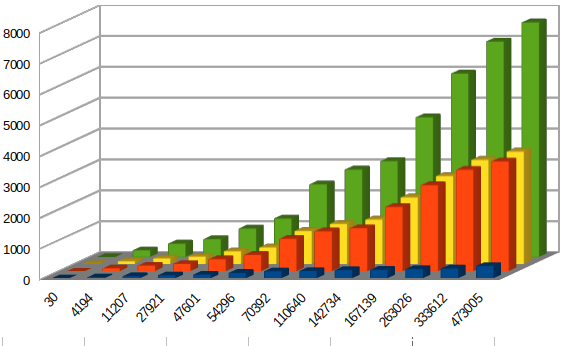
\includegraphics[width=\textwidth]{images/betoltesiido2.png}
\caption{Modell betöltési az egyes részeken grafikon.}
\label{fig:betolt2}
\end{figure}

\begin{itemize}
\item Kék színnel különböző adatok feltöltéséhez szükséges tömbök lefoglalása.
\item Narancssárga színnel lett jelölve a különböző változók összeszámlálása.
\item Sárga színnel lett jelölve az adatok tényleges kiolvasása a fájlból.
\item Grafikonon zöld színnel lett jelölve modell teljes betöltésének ideje.
 \end{itemize}
\bigskip
A grafikonról jól leolvasható, hogy a tömbök lefoglalása szinte jelentéktelen időt vesz igénybe a folyamat során. Változók összeszámlálása közel azonos időt vesz igénybe, mint a kiolvasás, ez azért van, mert mindkét folyamatnál végig kell menni a teljes OBJ fájl minden elemén.
